\chapter{Conclusion and Future Directions}

\section{Summary}

In \autoref{part:exchangeable}, I explored the potential of the double generalized linear model (DGLM) to detect novel QTL in linkage disequilibrium (LD) mapping experiments.
I described how the DGLM, unlike the standard linear model (SLM), can detect mean QTL, variance QTL, and joint mean-variance QTL.
This work was based on long-public, but little used statistical methods \citep{Smyth1989} applied to genetics experiments in a way that is relatively novel \citep{Pare2010,Ronnegard2011a}.
I extended previous work by developing a permutation approach that accurately controls the false positive rate (FPR) of an individual test to the desired level and can be applied naturally in a genome-wide context to accurately control the family-wise error rate (FWER).
Additionally, I developed novel plots for visualizing and interpreting the results of a genome scan based on these tests and have distributed software that implements this framework in \texttt{R} package \texttt{vqtl}, which is available on \texttt{CRAN} and is interoperable with the popular \texttt{R/qtl}.

I retrieved data from the Mouse Phenome Database to test my framework for QTL mapping with the DGLM and found three novel QTL.
In reanalyzing the data from \citet{Bailey2008}, I discovered a novel vQTL for rearing behavior, which was not detected previously because the standard analysis framework does not detect vQTL.
In reanalyzing the data from \citet{Kumar2013}, I discovered a novel mQTL for circadian behavior.
The additional power of the DGLM-based test to detect this QTL came from accommodating the variance heterogeneity across alleles at the QTL.
In reanalyzing the data from \citet{Leamy2000}, I discovered a novel mQTL for bodyweight at three weeks of age.
The additional power of the DGLM-based test to detect this QTL came from accommodating the variance heterogeneity across levels of a nuisance covariate --- which father sired the mouse on which the bodyweight was measured.
Gaining power to detect a QTL in this manner was novel and therefore I investigate the statistical power of DGLM-based tests in cases of what I've termed ``background variance heterogeneity''.
Simulations confirmed that when the source of variance heterogeneity is known, the DGLM-based tests for mQTL, vQTL, and mvQTL are uniquely powerful while maintaining accurate FPR control.


In \autoref{part:nonexchangeable}, I described the utility of the linear mixed model (LMM) for genetic mapping in non-exchangeable populations.
In such populations, both the SLM and the DGLM are inappropriate because they cannot account for the differential relatedness of individuals in the mapping population.
I described the established procedure for fitting the LMM that is fast enough to make genome-wide analysis tractable, and noted that one of its limitations is its requirement that the environmental variance be identical across all measurements.
I went on to report a novel mathematical method for rapidly fitting the LMM that allows for heteroskedastic residual variance, removing a limitation of the previous standard method.
I tested this method on simulated data and found it to have beneficial effects on FPR control and power to detect mQTL.
I have developed an \texttt{R} package that implements GWAS analysis using this method and it is available on \texttt{CRAN}.
The next step on this project is clear --- to apply the software to existing datasets to attempt to characterize the extent to which it changes the results of completed GWAS analyses and to potentially detect new QTL.


\section{Outstanding Specific Aims}

This dissertation to this point describes the results of aims 1a, 1b, and 2a.
Briefly, aim 1a was to accommodate variance heterogeneity in an LD mapping panel.
This aim was accomplished and its results were reported in the second reanalysis in \autoref{chap:mvqtl_reanalyses} and \autoref{chap:bvh}.
Aim 1b was to accommodate variance heterogeneity in an association mapping panel, and the results of that work are reported in \autoref{chap:het_LMM}.
Aim 2a was to identify variance heterogeneity in an LD mapping panel, which was reported in the first reanalysis in \autoref{chap:mvqtl_reanalyses}.
Here, I will discuss aims 2b and 3.

Aim 2b was to develop a statistical approach to detect vQTL in an inbred strain panel.
I began addressing this aim with a two-stage approach.
The first step was to use a Bayesian statistical modeling language like JAGS or STAN \citep{Plummer2003,Carpenter2017} to estimate the mean and variance of each strain.
The second intended step was to use a standard GWAS approach to detect genetic associations with those strain parameters.
Though I did not make meaningful progress on this work to date, I consider it a promising avenue of future research.

Aim 3 was to develop principled methods for combining evidence from LD mapping and association mapping panels.
With the benefit of three more years of study, I understand better the challenges that this aim faces.
Foremost among them is the question of how to reconcile the fact that a given genetic variant is likely to have drastically different effects depending on the genetic background in which it is expressed with the stated goal to share information across study designs.
Based on this challenge, I consider this aim to be a less-promising avenue for future research.


\section{Human Studies}

In the last two years, I worked on an exciting project to apply DGLM-based genetic mapping approaches to cardiovascular disease risk traits in humans.
I worked with Ethan and Leslie Lange and Laura Raffield, a postdoctoral researcher in their lab, to attempt to identify genetic loci that influence lipid levels and blood pressure traits.
This work did not achieve any meaningful results yet, but I believe it has tremendous potential to identify GxG and GxE interactions through the detection of vQTL.

The problem of differential relatedness was managed by including the first ten principle components of the genome as covariates in both the mean and variance sub-models.
This is a heuristic correction, and is less mathematically-sound than the application the linear mixed model described in \autoref{chap:het_LMM}.
Given the extremely large sample size involved in human GWAS studies, it is likely that even the efficient implementation of the LMM described here and elsewhere \citep{Kang2008} will not be tenable for the near future.
When I turned my focus away from this project and toward those that I completed, we were dealing with issues related to correction for $p$-value inflation with genomic control and how that might be different in the mean sub-model as compared to the variance sub-model.


% \section{QTL Mapping with Causally Ambiguous Covariates}

% In \autoref{part:exchangeable}, when using B as a mean or variance covariate for mapping A, we always assumed A was causally downstream of B, that no information flowed from B to A.
% For example, no phenotype influences which batch, housing, or sex a mouse is.
% In this setting, the value of including these covariates was clear --- it allowed the statistical model to identify patterns of variance heterogeneity and capitalize on them to increase the accuracy of the model to the data.

% Now, I consider cases where the flow of causality is ambiguous.
% What is the value in using B as a mean or variance covariate for mQTL or vQTL mapping?
% Using it as a mean or variance covariate
% WV and RC agree that using it as a variance covariate for mQTL mapping is probably a good thing -- gives weights that are more reflective of the true extent of residual variation.
% But what about the other 3 possibilities?
% There should be loads of literature on using it as a mean covariate for mQTL mapping -- trying to find some of that will be the next step for this section.


% \centering
% \begin{figure}
% 	\centering
% 	\begin{subfigure}{0.45\textwidth}
% 		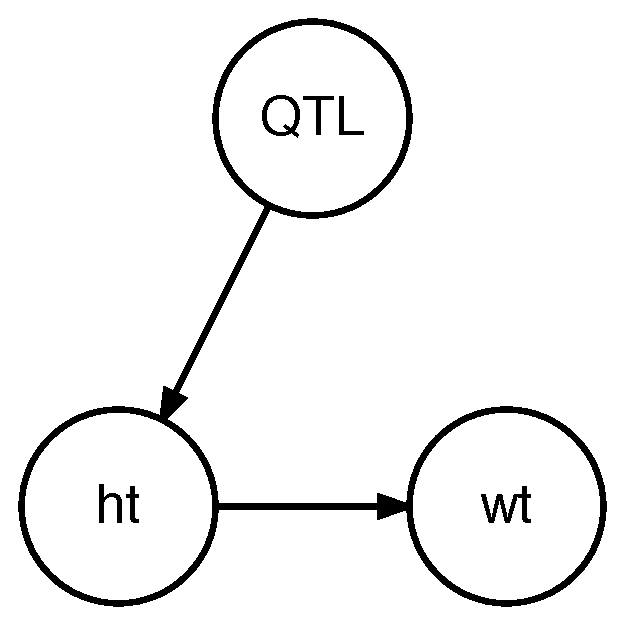
\includegraphics[width=0.8\linewidth]{images/graph_mm.pdf}
% 		\caption{Model MM: the QTL influences the mean of height and height influences the mean of weight.}
% 	\end{subfigure}\qquad
% 	\begin{subfigure}{0.45\textwidth}
% 		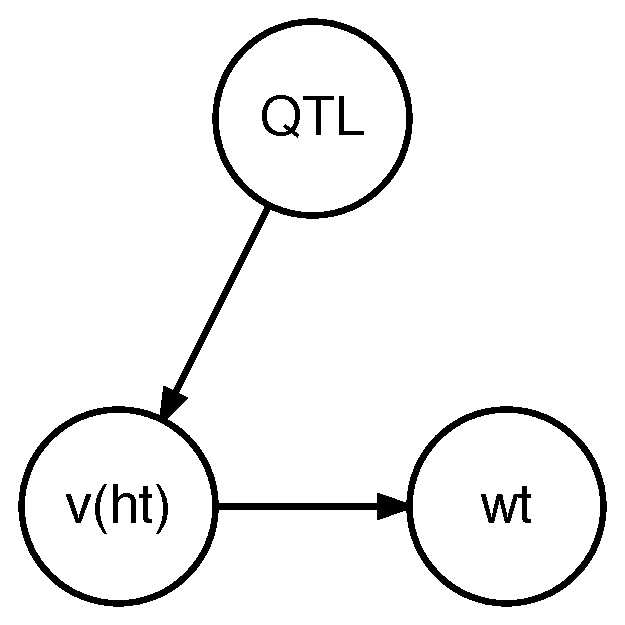
\includegraphics[width=0.8\linewidth]{images/graph_vm.pdf}
% 		\caption{Model VM: the QTL influences the variance of height and variance of height influences the mean of weight.}
% 	\end{subfigure}

% 	\vspace*{3em}
	
% 	\begin{subfigure}{0.45\textwidth}
% 		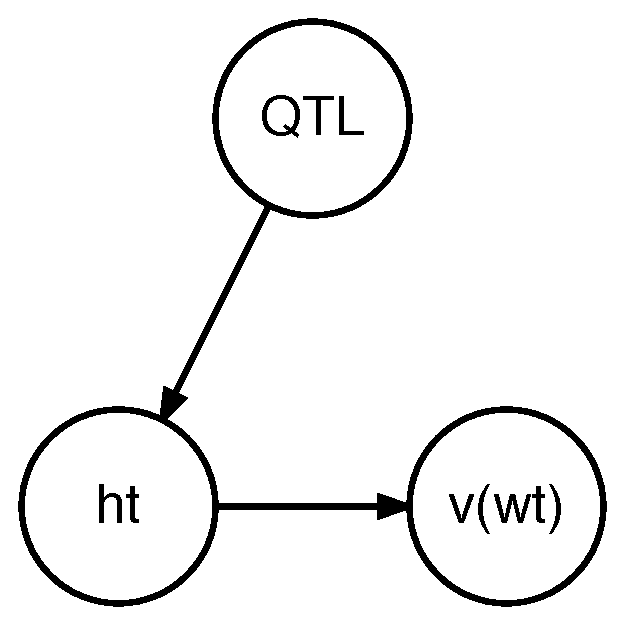
\includegraphics[width=0.8\linewidth]{images/graph_mv.pdf}
% 		\caption{Model MV: the QTL influences the mean of height and height influences the variance of weight.}
% 	\end{subfigure}\qquad
% 	\begin{subfigure}{0.45\textwidth}
% 		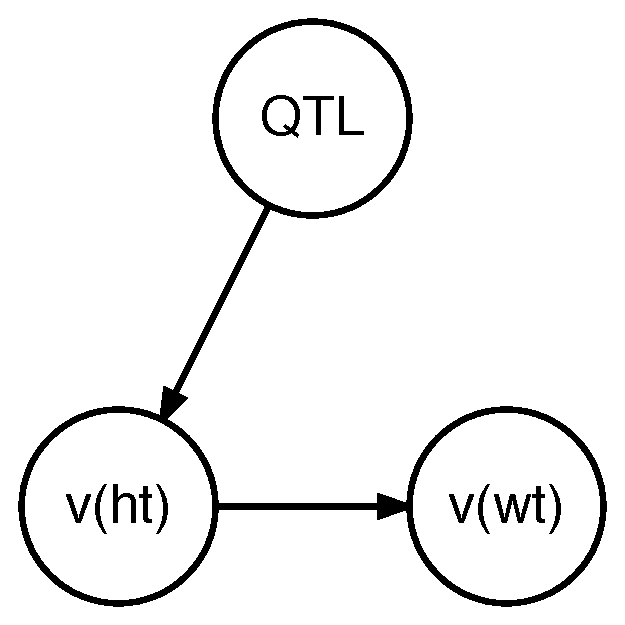
\includegraphics[width=0.8\linewidth]{images/graph_vv.pdf}
% 		\caption{Model VV: the QTL influences the variance of height and variance of height influences the variance of weight.}
% 	\end{subfigure}
% \end{figure}
